%! Author = Wiktor Rostkowski, Mateusz Budzisz
%! Date = 29/04/2024

\chapter{Projekt}
\label{ch:projekt}

\section{Wzorce projektowe}\label{sec:wzorce-projektowe}
W projekcie wykorzystano następujące wzorce projektowe:
\begin{itemize}

    \item \textbf{MVVM (Model-View-ViewModel)}: Wzorzec architektoniczny, który oddziela logikę biznesową (Model) od interfejsu użytkownika (View) za pomocą warstwy pośredniej (ViewModel), która zarządza stanem i logiką prezentacji.

    \item \textbf{MVC (Model-View-Controller)}: Wzorzec projektowy, który dzieli aplikację na trzy główne komponenty: Model (logika danych), View (interfejs użytkownika) i Controller (logika aplikacji).
    Pozwala to na lepsze zarządzanie kodem i jego modularność.

    \item \textbf{REST API (Representational State Transfer Application Programming Interface)}: Styl architektoniczny dla systemów rozproszonych, oparty na protokole HTTP, który umożliwia komunikację między klientem a serwerem za pomocą standardowych metod (GET, POST, PUT, DELETE).

    \item \textbf{Repository}: Wzorzec projektowy, który zapewnia warstwę abstrakcji nad dostępem do danych.
    Umożliwia oddzielenie logiki biznesowej od warstwy dostępu do danych, co ułatwia zarządzanie danymi i testowanie aplikacji.

    \item \textbf{Dependency Injection}: Technika polegająca na wstrzykiwaniu zależności do komponentów, zamiast tworzenia ich wewnątrz komponentów.
    Umożliwia to luźne powiązanie między komponentami i ułatwia testowanie oraz zarządzanie zależnościami.

    \item \textbf{Redux}: Wzorzec do zarządzania stanem aplikacji, szczególnie popularny w aplikacjach React.
    Opiera się na centralnym magazynie (store), który przechowuje cały stan aplikacji, oraz na akcjach i reduktorach, które modyfikują ten stan w kontrolowany sposób.

    \item \textbf{Observer}: Wzorzec projektowy, w którym obiekt (obserwowany) powiadamia inne obiekty (obserwatorów) o zmianach swojego stanu.
    Umożliwia to reaktywne programowanie i luźne powiązanie między obiektami.

    \item \textbf{Reverse Proxy}: Serwer pośredniczący, który przyjmuje żądania od klientów i przekazuje je do odpowiednich serwerów docelowych.
    Używany do zwiększenia wydajności, równoważenia obciążenia i poprawy bezpieczeństwa.

    \item \textbf{Bearer Token}: Metoda autoryzacji, w której token dostępu jest przesyłany w nagłówku HTTP\@.
    Umożliwia to bezpieczne uwierzytelnianie użytkowników i autoryzację dostępu do zasobów.

    \item \textbf{Service}: Pojęcie szerokie, odnoszące się do jednostki funkcjonalnej w aplikacji, która realizuje określoną usługę.

\end{itemize}

\section{Komponenty}\label{sec:komponenty}
W skład systemu wchodzą:
\begin{itemize}
    \item Internetowa aplikacja progresywna
    \item Backend zgodny ze standardem REST API
    \item Baza danych PostrgeSql
\end{itemize}

\section{Architektura}\label{sec:architektura}
System został zbudowany w architekturze monolitycznej, co oznacza, że wszystkie jego elementy i funkcjonalności są zintegrowane w jednym serwisie, zamiast być podzielone na niezależne moduły lub mikroserwisy.
System został wdrożony w chmurze obliczeniowej Oracle Ampere.
Aby uniknąć problemów z CORS (Cross-Origin Resource Sharing), wszystkie połączenia przychodzące z różnych źródeł są przekierowywane przez serwer Nginx.
Nginx działa jako reverse proxy, który odpowiednio kieruje ruch do właściwych komponentów systemu znajdujących się na serwerze.
Dzięki temu z perspektywy użytkownika wszystkie usługi systemu są dostępne pod tym samym adresem URL\@.
Dodatkowo, użycie Nginx umożliwia łatwe wygenerowanie certyfikatu SSL za pomocą Let's Encrypt, co zapewnia bezpieczne połączenia HTTPS i chroni dane użytkowników przed potencjalnymi zagrożeniami.

\begin{figure}[H]
    \centering
    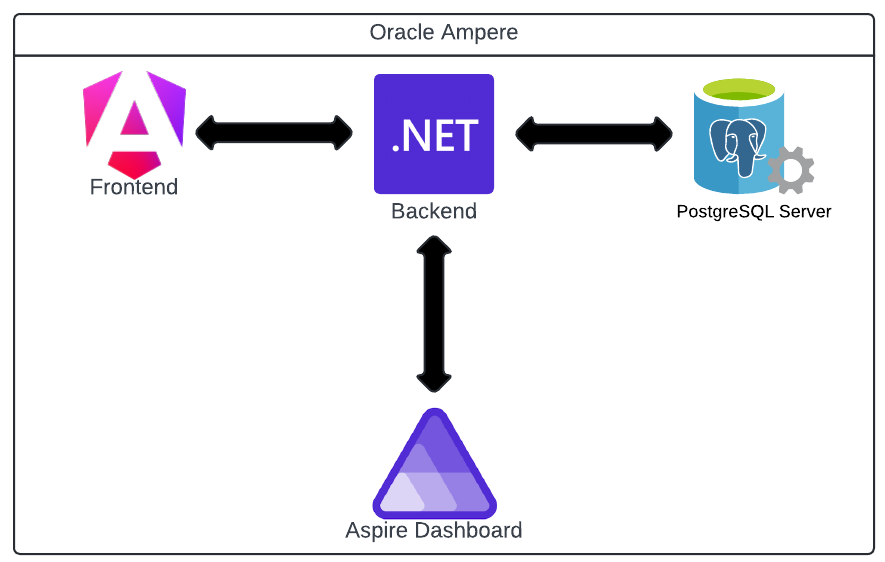
\includegraphics[width=1\textwidth]{attachments/arch-diag}
    \caption{Diagram systemu w środowisku docelowym}
    \label{fig:figure}
\end{figure}

\pagebreak
\subsection{Konfiguracja Nginx}
\label{subsec:konfiguracja-nginx}
Przedstawiona poniżej konfiguracja serwera NGINX zawiera definicje kilku serwerów wirtualnych dla różnych domen i usług.
Zamieszczono w niej szczegółowe wyjaśnienie każdego elementu konfiguracji.

\subsubsection{Główny serwer obsługujący \texttt{city-planner.budziszm.pl}}
\begin{longlisting}[language=nginx,label={lst:n1}]
server {
  server_name city-planner.budziszm.pl;

  root /var/www/city-planner.budziszm.pl/html;

  index index.html;
\end{longlisting}
\begin{itemize}
    \item \texttt{server\_name city-planner.budziszm.pl;}: Określa nazwę serwera, który obsługuje tę konfigurację.
    \item \texttt{root /var/www/city-planner.budziszm.pl/html;}: Ustala katalog główny dla plików serwowanych przez ten serwer.
    \item \texttt{index index.html;}: Ustawia domyślny plik indeksu.
\end{itemize}

\begin{longlisting}[language=nginx,label={lst:n2}]
  location = /favicon.ico { access_log off; log_not_found off; }
\end{longlisting}
\begin{itemize}
    \item \texttt{location = /favicon.ico}: Reguła dla \texttt{favicon.ico}.
    Wyłącza logowanie dostępu oraz błędów, jeśli plik nie zostanie znaleziony.
\end{itemize}

\subsubsection{Konfiguracja gzip}
\begin{longlisting}[language=nginx,label={lst:n3}]
  gzip on;
  gzip_static on;
  gzip_types
    text/plain
    text/css
    text/js
    text/xml
    text/javascript
    application/javascript
    application/json
    application/xml
    application/rss+xml
    image/svg+xml;
  gzip_proxied no-cache no-store private expired auth;
\end{longlisting}
\begin{itemize}
    \item \texttt{gzip on;} i \texttt{gzip\_static on;}: Włącza kompresję gzip i kompresję statyczną.
    \item \texttt{gzip\_types}: Określa typy MIME, które mają być kompresowane.
    \item \texttt{gzip\_proxied}: Definiuje warunki, pod którymi odpowiedzi z proxy mogą być kompresowane.
\end{itemize}

\subsubsection{Konfiguracja cache dla CSS i JS}
\begin{longlisting}[language=nginx,label={lst:n4}]
  location ~*.(css|js)$ {
    add_header Cache-Control "public, immutable, max-age=31536000";
  }
\end{longlisting}
\begin{itemize}
    \item \texttt{location ~*.(css|js)\$}: Obsługuje wszystkie pliki CSS i JS@.
    \item \texttt{add\_header Cache-Control "public, immutable, max-age=31536000";}: Dodaje nagłówek kontrolujący cache, który umożliwia przechowywanie plików w pamięci podręcznej przez rok.
\end{itemize}

\subsubsection{Przekierowania proxy dla \texttt{/Api} i \texttt{/confirmEmail}}
\begin{longlisting}[language=nginx,label={lst:n5}]
  location /Api {
    rewrite /Api/(.*) /$1 break;
    proxy_pass http://localhost:5000;
    proxy_redirect off;
    proxy_set_header Host $host;
  }

  location /confirmEmail {
    proxy_pass http://localhost:5000;
    proxy_redirect off;
    proxy_set_header Host $host;
  }
\end{longlisting}
\begin{itemize}
    \item \texttt{location /Api} i \texttt{location /confirmEmail}: Przekierowują żądania na odpowiednie endpointy do lokalnego serwera działającego na porcie 5000.
\end{itemize}

\subsubsection{Obsługa plików w \texttt{/thesis}}
\begin{longlisting}[language=nginx,label={lst:n6}]
  location ~* /thesis/(.*)$ {
    root /opt/city-planner-documentation;
    rewrite /thesis/(.*) /$1.pdf break;
    add_header Content-Disposition 'inline';
    try_files $uri =404;
  }

  location /thesis {
    root /opt/city-planner-documentation;
    rewrite /thesis /thesis.pdf break;
    add_header Content-Disposition 'inline';
    try_files $uri =404;
  }
\end{longlisting}
\begin{itemize}
    \item Obsługuje dostęp do plików w katalogu \texttt{/opt/city-planner-documentation}, zmieniając ścieżki i dodając nagłówek \texttt{Content-Disposition} do wyświetlania plików PDF w przeglądarce.
\end{itemize}

\subsubsection{Główne ustawienia dla ścieżek i SSL}
\begin{longlisting}[language=nginx,label={lst:n7}]
  location / {
    try_files $uri$args $uri$args/ /index.html;
  }

  listen 443 ssl; # managed by Certbot
  ssl_certificate /etc/letsencrypt/live/city-planner.budziszm.pl/fullchain.pem; # managed by Certbot
  ssl_certificate_key /etc/letsencrypt/live/city-planner.budziszm.pl/privkey.pem; # managed by Certbot
  include /etc/letsencrypt/options-ssl-nginx.conf; # managed by Certbot
  ssl_dhparam /etc/letsencrypt/ssl-dhparams.pem; # managed by Certbot
\end{longlisting}
\begin{itemize}
    \item \texttt{location /}: Przekierowuje do pliku \texttt{index.html} jeśli plik lub katalog nie zostaną znalezione.
    \item \texttt{listen 443 ssl;}: Konfiguruje serwer do nasłuchiwania na porcie 443 z SSL\@.
    \item \texttt{ssl\_certificate}, \texttt{ssl\_certificate\_key}, \texttt{include}, \texttt{ssl\_dhparam}: Konfiguracja SSL przy użyciu certyfikatów Let's Encrypt.
\end{itemize}

\subsubsection{Przekierowanie HTTP do HTTPS}
\begin{longlisting}[language=nginx,label={lst:n8}]
server {
    if ($host = city-planner.budziszm.pl) {
        return 301 https://$host$request_uri;
    } # managed by Certbot

    server_name city-planner.budziszm.pl;
    listen 80;
    return 404; # managed by Certbot
}
\end{longlisting}
\begin{itemize}
    \item Przekierowuje ruch HTTP na HTTPS dla \texttt{city-planner.budziszm.pl}.
\end{itemize}

\subsubsection{Serwer obsługujący \texttt{logs.city-planner.budziszm.pl}}
\begin{longlisting}[language=nginx,label={lst:n9}]
server {
  server_name logs.city-planner.budziszm.pl;
  auth_basic           "Administrator's Area";
  auth_basic_user_file /etc/apache2/.htpasswd;
  error_log  /var/log/nginx/error.log debug;

  location / {
    proxy_pass https://localhost:18888;
    proxy_redirect off;
    proxy_http_version 1.1;
    proxy_set_header Upgrade $http_upgrade;
    proxy_set_header Connection "Upgrade";
    proxy_set_header Host $host;
  }

  listen 443 ssl; # managed by Certbot
  ssl_certificate /etc/letsencrypt/live/city-planner.budziszm.pl/fullchain.pem; # managed by Certbot
  ssl_certificate_key /etc/letsencrypt/live/city-planner.budziszm.pl/privkey.pem; # managed by Certbot
  include /etc/letsencrypt/options-ssl-nginx.conf; # managed by Certbot
  ssl_dhparam /etc/letsencrypt/ssl-dhparams.pem; # managed by Certbot
}
\end{longlisting}
\begin{itemize}
    \item Obsługuje ruch na \texttt{logs.city-planner.budziszm.pl} z podstawową autoryzacją.
    \item Przekierowuje ruch do lokalnego serwera na porcie 18888 z obsługą WebSocketów.
\end{itemize}

\subsubsection{Przekierowanie HTTP do HTTPS dla \texttt{logs.city-planner.budziszm.pl}}
\begin{longlisting}[language=nginx,label={lst:n10}]
server {
    if ($host = logs.city-planner.budziszm.pl) {
        return 301 https://$host$request_uri;
    } # managed by Certbot

    listen 80;
    server_name logs.city-planner.budziszm.pl;
    return 404; # managed by Certbot
}
\end{longlisting}
\begin{itemize}
    \item Przekierowuje ruch HTTP na HTTPS dla \texttt{logs.city-planner.budziszm.pl}.
\end{itemize}

\subsubsection{Mapowanie nagłówka \texttt{Connection} w zależności od nagłówka \texttt{Upgrade}}
\begin{longlisting}[language=nginx,label={lst:n11}]
map $http_upgrade $connection_upgrade {
  default upgrade;
  ''      close;
}
\end{longlisting}
\begin{itemize}
    \item Ustawia wartość nagłówka \texttt{Connection} w zależności od obecności nagłówka \texttt{Upgrade}.
    Umożliwia to poprawne działanie WebSocketów.
\end{itemize}

Ta konfiguracja zapewnia pełną obsługę zarówno dla serwowania statycznych stron, jak i przekierowania ruchu do usług backendowych, zapewniając jednocześnie bezpieczeństwo przez użycie SSL i kontrolę cache dla plików statycznych.

\subsection{Deployment backendu}
\label{subsec:deployment-backendu}
Ten skrypt Bash wykonuje kilka kroków, aby wdrożyć backend aplikacji.
Poniżej znajduje się szczegółowy opis, co robi każda jego część:

\subsubsection{Usuwanie wszystkich plików z /opt/city-planner-backend/publish}
Ten krok usuwa wszystkie pliki z katalogu \texttt{/opt/city-planner-backend/publish}, aby przygotować miejsce na nowe pliki.
\begin{longlisting}[style=shell-colored,label={lst:db1}]
+echo+ "Removing all files from /opt/city-planner-backend/publish"
+rm -Rf+ /opt/city-planner-backend/publish/*
\end{longlisting}

\subsubsection{Kopiowanie plików do /opt/city-planner-backend/publish/}
Ten krok kopiuje opublikowane pliki z katalogu \texttt{WebApi/bin/production/net8.0/linux-arm64/publish/} do \texttt{/opt/city-planner-backend/publish/}.
\begin{longlisting}[style=shell-colored,label={lst:db2}]
+echo+ "Copying publish files to /opt/city-planner-backend/publish/"
+cp+ WebApi/bin/production/net8.0/linux-arm64/publish/* /opt/city-planner-backend/publish/
\end{longlisting}

\subsubsection{Przygotowanie pliku usługi SystemD}
Ten krok tworzy nowy plik usługi SystemD dla backendu aplikacji.
Plik usługi zawiera konfigurację dla SystemD, w tym opis, zależności, ustawienia serwisu i polecenie uruchomienia.

\begin{longlisting}[style=shell-colored,label={lst:db3}]
+echo+ "Preparing SystemD service file"
+rm -f+ /etc/systemd/system/city-planner-backend.service
+cat+ <<EOT >> /etc/systemd/system/city-planner-backend.service
[Unit]
Description=City planner backend
After=network.target
StartLimitIntervalSec=0

[Service]
Type=simple
Restart=always
RestartSec=1
User=ubuntu
EnvironmentFile=/opt/city-planner-backend/environment.conf
WorkingDirectory=/opt/city-planner-backend/publish
ExecStart=/opt/city-planner-backend/publish/WebApi

[Install]
WantedBy=multi-user.target
EOT
\end{longlisting}

\subsubsection{Włączanie pliku usługi SystemD}
Ten krok włącza nowo utworzony plik usługi SystemD, aby uruchamiał się automatycznie przy starcie systemu.
\begin{longlisting}[style=shell-colored,label={lst:db4}]
+echo+ "Enabling SystemD service file"
+systemctl enable+ city-planner-backend
\end{longlisting}

\subsubsection{Restartowanie usługi SystemD}
Ten krok restartuje usługę SystemD, aby zastosować nowe ustawienia i uruchomić backend aplikacji.
\begin{longlisting}[style=shell-colored,label={lst:db5}]
+echo+ "Restarting SystemD service file"
+systemctl restart+ city-planner-backend
\end{longlisting}

\subsubsection{Zakończenie wdrożenia backendu}
Ten krok wyświetla komunikat informujący o zakończeniu wdrożenia backendu.
\begin{longlisting}[style=shell-colored,label={lst:db6}]
+echo+ "Backend deployment done"
\end{longlisting}

\subsubsection{Całość kodu}
\begin{longlisting}[style=shell-colored,label={lst:db7}]
#!/bin/bash

+echo+ "Removing all files from /opt/city-planner-backend/publish"
+rm -Rf+ /opt/city-planner-backend/publish/*

+echo+ "Copying publish files to /opt/city-planner-backend/publish/"
+cp+ WebApi/bin/production/net8.0/linux-arm64/publish/* /opt/city-planner-backend/publish/
+echo+ "Preparing SystemD service file"
+rm -f+ /etc/systemd/system/city-planner-backend.service
+cat+ <<EOT >> /etc/systemd/system/city-planner-backend.service
[Unit]
Description=City planner backend
After=network.target
StartLimitIntervalSec=0

[Service]
Type=simple
Restart=always
RestartSec=1
User=ubuntu
EnvironmentFile=/opt/city-planner-backend/environment.conf
WorkingDirectory=/opt/city-planner-backend/publish
ExecStart=/opt/city-planner-backend/publish/WebApi

[Install]
WantedBy=multi-user.target
EOT

+echo+ "Enabling SystemD service file"
+systemctl enable+ city-planner-backend
+echo+ "Restarting SystemD service file"
+systemctl restart+ city-planner-backend

+echo+ "Backend deployment done"
\end{longlisting}

\subsection{Deployment frontendu}
Ten skrypt Bash wykonuje kilka kroków, aby wdrożyć frontend aplikacji.
Poniżej znajduje się szczegółowy opis, co robi każda jego część:

\subsubsection{Usuwanie wszystkich plików z \newline
/var/www/city-planner.budziszm.pl/html}
Ten krok usuwa wszystkie pliki z katalogu \texttt{/var/www/city-planner.budziszm.pl/html}, aby przygotować miejsce na nowe pliki.
\begin{longlisting}[style=shell-colored]
+echo+ "Removing all files from /var/www/city-planner.budziszm.pl/html"
+rm -Rf+ /var/www/city-planner.budziszm.pl/html/*
\end{longlisting}

\subsubsection{Kopiowanie plików do /var/www/city-planner.budziszm.pl/html/}
Ten krok kopiuje pliki z katalogu \texttt{dist/frontend/browser/} \newline
do \texttt{/var/www/city-planner.budziszm.pl/html/}.
\begin{longlisting}[style=shell-colored]
+echo+ "Copying dist files to /var/www/city-planner.budziszm.pl/html/"
+cp -r+ dist/frontend/browser/* /var/www/city-planner.budziszm.pl/html/
\end{longlisting}

\subsubsection{Zakończenie wdrożenia frontendu}
Ten krok wyświetla komunikat informujący o zakończeniu wdrożenia frontendu.
\begin{longlisting}[style=shell-colored]
+echo+ "Frontend deployment done"
\end{longlisting}

\subsubsection{Całość kodu}
\begin{longlisting}[style=shell-colored]
#!/bin/bash

+echo+ "Removing all files from /var/www/city-planner.budziszm.pl/html"
+rm -Rf+ /var/www/city-planner.budziszm.pl/html/*

+echo+ "Copying dist files to /var/www/city-planner.budziszm.pl/html/"
+cp -r+ dist/frontend/browser/* /var/www/city-planner.budziszm.pl/html/

+echo+ "Frontend deployment done"
\end{longlisting}

\section{Specyfikacja API}
Do implementacji API został użyty framework ASP.NET 8, który umożliwia tworzenie wydajnych i skalowalnych aplikacji webowych. Do zarządzania warstwą dostępu do danych i mapowania obiektowo-relacyjnego (ORM) zastosowano Entity Framework, w połączeniu z biblioteką Npgsql, która pozwala na efektywną współpracę z bazą danych PostgreSQL\@.
Dzięki temu rozwiązaniu możliwe było stworzenie solidnej i wydajnej aplikacji z wykorzystaniem nowoczesnych technologii .NET, zapewniając jednocześnie łatwość w zarządzaniu danymi i wysoką kompatybilność z relacyjnymi bazami danych.

W trakcie prac do prezentacji dokumentacji endpointów użyto Swaggera i ReDoca.

\begin{figure}[H]
\centering
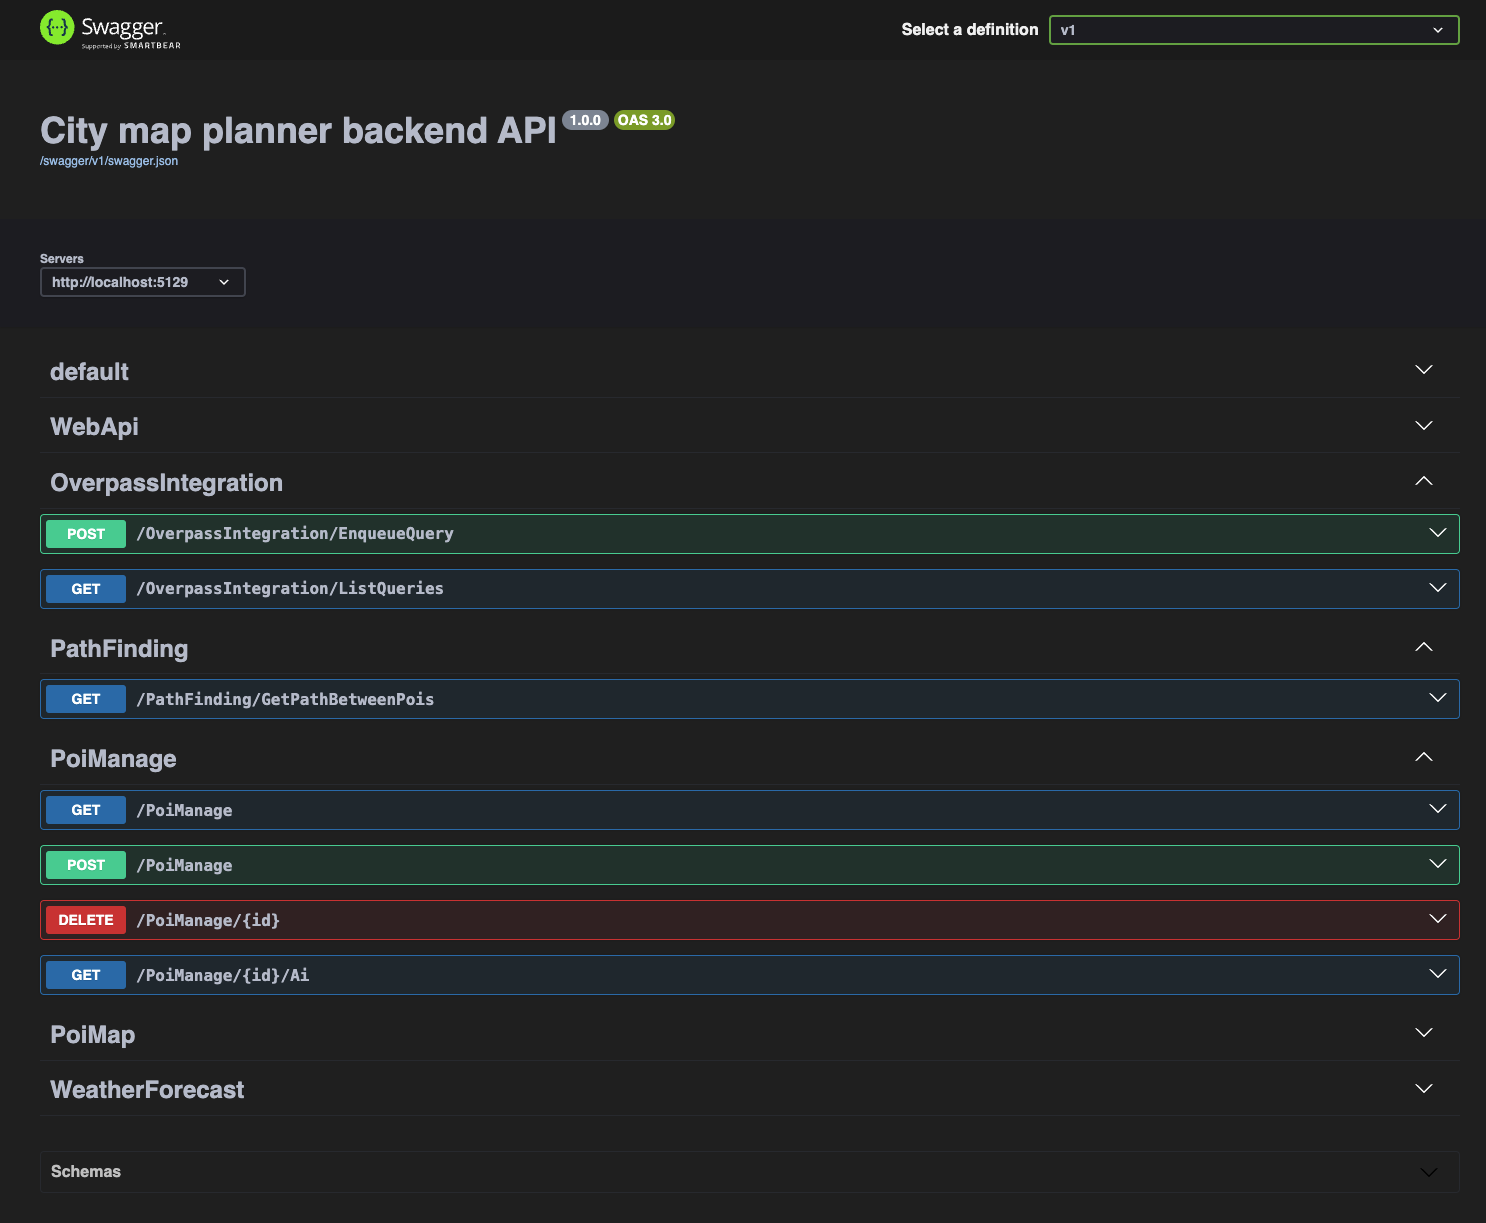
\includegraphics[width=1\textwidth]{attachments/swagger}
\caption{Dokumentacji API w programie Swagger}
\label{fig:figure}
\end{figure}

\begin{figure}[H]
\centering

\includegraphics[width=1\textwidth]{attachments/redoc}
\caption{Dokumentacji API w programie ReDoc}
\label{fig:figure}
\end{figure}

Poniżej przedstawiono specyfikację dostępnych punktów końcowych:

\subsection{Autoryzacja i zarządzanie użytkownikami}
\subsubsection{\lstinline[language=http]{POST /register}}
Rejestracja nowego użytkownika. \\
\textbf{Request body:}
\begin{lstlisting}[language=json]
{
  "email": "string",
  "password": "string"
}
\end{lstlisting}
\textbf{Responses:}
\begin{itemize}
    \item 200: Rejestracja powiodła się.
    \item 400: Błąd walidacji danych.
\begin{lstlisting}[language=json]
{
  "type": "string",
  "title": "string",
  "status": 0,
  "detail": "string",
  "instance": "string",
  "errors": {
    "additionalProp1": [
      "string"
    ],
    "additionalProp2": [
      "string"
    ],
    "additionalProp3": [
      "string"
    ]
  }
}
\end{lstlisting}
\end{itemize}

\subsubsection{\lstinline[language=http]{POST /login}}
Logowanie użytkownika. \\
\textbf{Query parameters:}
\begin{itemize}
    \item \texttt{useCookies} (boolean, opcjonalny)
    \item \texttt{useSessionCookies} (boolean, opcjonalny)
\end{itemize}
\textbf{Request body:}
\begin{lstlisting}[language=json]
{
  "email": "string",
  "password": "string",
  "twoFactorCode": "string",
  "twoFactorRecoveryCode": "string"
}
\end{lstlisting}
\textbf{Responses:}
\begin{itemize}
    \item 200:
\begin{lstlisting}[language=json]
{
  "tokenType": "string",
  "accessToken": "string",
  "expiresIn": 0,
  "refreshToken": "string"
}
\end{lstlisting}
\end{itemize}

\subsubsection{\lstinline[language=http]{POST /refresh}}
Odświeżenie tokenu autoryzacyjnego. \\
\textbf{Request body:}
\begin{lstlisting}[language=json]
{
  "refreshToken": "string"
}
\end{lstlisting}
\textbf{Responses:}
\begin{itemize}
    \item 200:
\begin{lstlisting}[language=json]
{
  "tokenType": "string",
  "accessToken": "string",
  "expiresIn": 0,
  "refreshToken": "string"
}
\end{lstlisting}
\end{itemize}

\subsubsection{\lstinline[language=http]{GET /confirmEmail}}
Potwierdzenie adresu email. \\
\textbf{Query parameters:}
\begin{itemize}
    \item \texttt{userId} (string, opcjonalny)
    \item \texttt{code} (string, opcjonalny)
    \item \texttt{changedEmail} (string, opcjonalny)
\end{itemize}
\textbf{Responses:}
\begin{itemize}
    \item 200: Potwierdzenie zakończone sukcesem.
\end{itemize}

\subsubsection{\lstinline[language=http]{POST /resendConfirmationEmail}}
Ponowne wysłanie emaila z potwierdzeniem. \\
\textbf{Request body:}
\begin{lstlisting}[language=json]
{
  "email": "string"
}
\end{lstlisting}
\textbf{Responses:}
\begin{itemize}
    \item 200: Email z potwierdzeniem wysłany ponownie.
\end{itemize}

\subsubsection{\lstinline[language=http]{POST /forgotPassword}}
Przypomnienie hasła. \\
\textbf{Request body:}
\begin{lstlisting}[language=json]
{
  "email": "string"
}
\end{lstlisting}
\textbf{Responses:}
\begin{itemize}
    \item 200: Email z instrukcjami wysłany.
    \item 400:
\begin{lstlisting}[language=json]
{
  "type": "string",
  "title": "string",
  "status": 0,
  "detail": "string",
  "instance": "string",
  "errors": {
    "additionalProp1": [
      "string"
    ],
    "additionalProp2": [
      "string"
    ],
    "additionalProp3": [
      "string"
    ]
  }
}
\end{lstlisting}
\end{itemize}

\subsubsection{\lstinline[language=http]{POST /resetPassword}}
Resetowanie hasła. \\
\textbf{Request body:}
\begin{lstlisting}[language=json]
{
  "email": "string",
  "resetCode": "string",
  "newPassword": "string"
}
\end{lstlisting}
\textbf{Responses:}
\begin{itemize}
    \item 200: Hasło zresetowane.
    \item 400:
\begin{lstlisting}[language=json]
{
  "type": "string",
  "title": "string",
  "status": 0,
  "detail": "string",
  "instance": "string",
  "errors": {
    "additionalProp1": [
      "string"
    ],
    "additionalProp2": [
      "string"
    ],
    "additionalProp3": [
      "string"
    ]
  }
}
\end{lstlisting}
\end{itemize}

\subsubsection{\lstinline[language=http]{POST /manage/2fa}}
Zarządzanie dwuskładnikowym uwierzytelnianiem (2FA). \\
\textbf{Request body:}
\begin{lstlisting}[language=json]
{
  "enable": true,
  "twoFactorCode": "string",
  "resetSharedKey": true,
  "resetRecoveryCodes": true,
  "forgetMachine": true
}
\end{lstlisting}
\textbf{Responses:}
\begin{itemize}
    \item 200:
\begin{lstlisting}[language=json]
{
  "sharedKey": "string",
  "recoveryCodesLeft": 0,
  "recoveryCodes": [
    "string"
  ],
  "isTwoFactorEnabled": true,
  "isMachineRemembered": true
}
\end{lstlisting}
    \item 400:
\begin{lstlisting}[language=json]
{
  "type": "string",
  "title": "string",
  "status": 0,
  "detail": "string",
  "instance": "string",
  "errors": {
    "additionalProp1": [
      "string"
    ],
    "additionalProp2": [
      "string"
    ],
    "additionalProp3": [
      "string"
    ]
  }
}
\end{lstlisting}
    \item 404: Nie znaleziono zasobu.
\end{itemize}

\subsubsection{\lstinline[language=http]{GET /manage/info}}
Pobranie informacji o koncie. \\
\textbf{Responses:}
\begin{itemize}
    \item 200:
\begin{lstlisting}[language=json]
{
  "email": "string",
  "isEmailConfirmed": true
}
\end{lstlisting}
    \item 400:
\begin{lstlisting}[language=json]
{
  "type": "string",
  "title": "string",
  "status": 0,
  "detail": "string",
  "instance": "string",
  "errors": {
    "additionalProp1": [
      "string"
    ],
    "additionalProp2": [
      "string"
    ],
    "additionalProp3": [
      "string"
    ]
  }
}
\end{lstlisting}
    \item 404: Nie znaleziono zasobu.
\end{itemize}

\subsubsection{\lstinline[language=http]{POST /manage/info}}
Aktualizacja informacji o koncie. \\
\textbf{Request body:}
\begin{lstlisting}[language=json]
{
  "newEmail": "string",
  "newPassword": "string",
  "oldPassword": "string"
}
\end{lstlisting}
\textbf{Responses:}
\begin{itemize}
    \item 200:
\begin{lstlisting}[language=json]
{
  "email": "string",
  "isEmailConfirmed": true
}
\end{lstlisting}
    \item 400:
\begin{lstlisting}[language=json]
{
  "type": "string",
  "title": "string",
  "status": 0,
  "detail": "string",
  "instance": "string",
  "errors": {
    "additionalProp1": [
      "string"
    ],
    "additionalProp2": [
      "string"
    ],
    "additionalProp3": [
      "string"
    ]
  }
}
\end{lstlisting}
    \item 404: Nie znaleziono zasobu.
\end{itemize}

\subsubsection{\lstinline[language=http]{POST /logout}}
Wylogowanie użytkownika. \\
\textbf{Request body:} Pusty JSON \\
\textbf{Responses:}
\begin{itemize}
    \item 200: Wylogowanie zakończone sukcesem.
\end{itemize}

\subsubsection{\lstinline[language=http]{GET /exists}}
Sprawdzenie czy email istnieje w systemie. \\
\textbf{Query parameters:}
\begin{itemize}
    \item \texttt{email} (string, wymagany)
\end{itemize}
\textbf{Responses:}
\begin{itemize}
    \item 200: Email istnieje.
\end{itemize}

\subsubsection{\lstinline[language=http]{POST /deleteMe}}
Usunięcie konta użytkownika. \\
\textbf{Responses:}
\begin{itemize}
    \item 200: Konto usunięte.
\end{itemize}

\subsection{Integracja z Overpass}

\subsubsection{\lstinline[language=http]{POST /OverpassIntegration/EnqueueQuery}}
Kolejkowanie zapytania Overpass. \\
\textbf{Responses:}
\begin{itemize}
    \item 200: Zapytanie dodane do kolejki.
\end{itemize}

\subsubsection{\lstinline[language=http]{GET /OverpassIntegration/ListQueries}}
Pobranie listy zapytań Overpass. \\
\textbf{Responses:}
\begin{lstlisting}[language=json]
[
  "string"
]
\end{lstlisting}
\begin{itemize}
    \item 401: Nieautoryzowany dostęp.
\end{itemize}

\subsection{Zarządzanie Punktami POI}

\subsubsection{\lstinline[language=http]{GET /PoiManage}}
Pobranie listy punktów POI. \\
\textbf{Responses:}
\begin{lstlisting}[language=json]
[
  {
    "id": 0,
    "name": "string",
    "description": "string",
    "modified": "2023-01-01T00:00:00Z",
    "businessHoursPageUrl": "string",
    "businessHoursPageXPath": "string",
    "businessHoursPageModified": "2023-01-01T00:00:00Z",
    "holidaysPageUrl": "string",
    "holidaysPageXPath": "string",
    "holidaysPageModified": "2023-01-01T00:00:00Z",
    "entrances": [
      {
        "osmNodeId": 0,
        "name": "string",
        "description": "string"
      }
    ],
    "images": [
      {
        "fullSrc": "string",
        "iconSrc": "string",
        "attribution": "string"
      }
    ],
    "preferredWmoCodes": [
      0
    ],
    "preferredSightseeingTime": "string",
    "businessTimes": [
      {
        "effectiveFrom": "2023-01-01T00:00:00Z",
        "effectiveTo": "2023-01-01T00:00:00Z",
        "effectiveDays": [
          0
        ],
        "timeFrom": "00:00:00",
        "timeTo": "00:00:00",
        "state": 0
      }
    ]
  }
]
\end{lstlisting}

\subsubsection{\lstinline[language=http]{POST /PoiManage}}
Dodanie lub aktualizacja punktu POI. \\
\textbf{Request body:}
\begin{lstlisting}[language=json]
{
  "id": 0,
  "name": "string",
  "description": "string",
  "modified": "2023-01-01T00:00:00Z",
  "businessHoursPageUrl": "string",
  "businessHoursPageXPath": "string",
  "businessHoursPageModified": "2023-01-01T00:00:00Z",
  "holidaysPageUrl": "string",
  "holidaysPageXPath": "string",
  "holidaysPageModified": "2023-01-01T00:00:00Z",
  "entrances": [
    {
      "osmNodeId": 0,
      "name": "string",
      "description": "string"
    }
  ],
  "images": [
    {
      "fullSrc": "string",
      "iconSrc": "string",
      "attribution": "string"
    }
  ],
  "preferredWmoCodes": [
    0
  ],
  "preferredSightseeingTime": "string",
  "businessTimes": [
    {
      "effectiveFrom": "2023-01-01T00:00:00Z",
      "effectiveTo": "2023-01-01T00:00:00Z",
      "effectiveDays": [
        0
      ],
      "timeFrom": "00:00:00",
      "timeTo": "00:00:00",
      "state": 0
    }
  ]
}
\end{lstlisting}
\textbf{Responses:}
\begin{lstlisting}[language=json]
{
  "id": 0,
  "name": "string",
  "description": "string",
  "modified": "2023-01-01T00:00:00Z",
  "businessHoursPageUrl": "string",
  "businessHoursPageXPath": "string",
  "businessHoursPageModified": "2023-01-01T00:00:00Z",
  "holidaysPageUrl": "string",
  "holidaysPageXPath": "string",
  "holidaysPageModified": "2023-01-01T00:00:00Z",
  "entrances": [
    {
      "osmNodeId": 0,
      "name": "string",
      "description": "string"
    }
  ],
  "images": [
    {
      "fullSrc": "string",
      "iconSrc": "string",
      "attribution": "string"
    }
  ],
  "preferredWmoCodes": [
    0
  ],
  "preferredSightseeingTime": "string",
  "businessTimes": [
    {
      "effectiveFrom": "2023-01-01T00:00:00Z",
      "effectiveTo": "2023-01-01T00:00:00Z",
      "effectiveDays": [
        0
      ],
      "timeFrom": "00:00:00",
      "timeTo": "00:00:00",
      "state": 0
    }
  ]
}
\end{lstlisting}

\subsubsection{\lstinline[language=http]{DELETE /PoiManage/\{id\}}}
Usunięcie punktu POI. \\
\textbf{Path parameters:}
\begin{itemize}
    \item \texttt{id} (integer, wymagany)
\end{itemize}
\textbf{Responses:}
\begin{itemize}
    \item 200: Punkt POI usunięty.
\end{itemize}

\subsubsection{\lstinline[language=http]{GET /PoiManage/\{id\}/Ai}}
Pobranie informacji AI dla punktu POI. \\
\textbf{Path parameters:}
\begin{itemize}
    \item \texttt{id} (integer, wymagany)
\end{itemize}
\textbf{Responses:}
\begin{lstlisting}[language=json]
[
  {
    "effectiveFrom": "2023-01-01T00:00:00Z",
    "effectiveTo": "2023-01-01T00:00:00Z",
    "effectiveDays": [
      0
    ],
    "timeFrom": "00:00:00",
    "timeTo": "00:00:00",
    "state": 0
  }
]
\end{lstlisting}

\subsection{Mapowanie Punktów POI}

\subsubsection{\lstinline[language=http]{GET /PoiMap/List}}
Lista punktów POI na mapie. \\
\textbf{Responses:}
\begin{lstlisting}[language=json]
[
  {
    "id": 0,
    "map": {
      "label": "string",
      "iconSrc": "string",
      "lat": 0,
      "lon": 0
    },
    "details": {
      "bannerSrc": "string",
      "title": "string",
      "description": "string"
    },
    "preferredSightseeingTime": "string",
    "businessHours": [
      {
        "effectiveFrom": "2023-01-01T00:00:00Z",
        "effectiveTo": "2023-01-01T00:00:00Z",
        "effectiveDays": [
          0
        ],
        "timeFrom": "00:00:00",
        "timeTo": "00:00:00",
        "state": 0
      }
    ]
  }
]
\end{lstlisting}

\subsubsection{\lstinline[language=http]{GET /WeatherForecast}}
Pobranie prognozy pogody. \\
\textbf{Responses:}
\begin{lstlisting}[language=json]
[
  {
    "date": "2023-01-01",
    "temperatureC": 0,
    "temperatureF": 0,
    "summary": "string"
  }
]
\end{lstlisting}

\section{Baza danych}
Baza danych została podzielona na dwa schematy: \texttt{data} oraz \texttt{user\_data}, aby lepiej zarządzać różnymi rodzajami informacji.
Schemat \texttt{data} zawiera informacje o atrakcjach turystycznych oraz mapie miasta, które są dostępne publicznie.
Dane te mogą obejmować opisy zabytków, godziny otwarcia, lokalizacje na mapie oraz inne informacje przydatne dla turystów.
Z kolei schemat \texttt{user\_data} przechowuje tylko dane logowania oraz uprawnienia użytkowników.
Taki podział pozwala na lepsze zabezpieczenie danych użytkowników, usprawnienie zarządzania bazą danych oraz łatwiejsze stosowanie różnych poziomów dostępu i kontroli nad danymi.
Tabele posiadają różnorodne klucze obce, które zapewniają integralność danych poprzez powiązania między tabelami oraz mechanizm kaskadowego usuwania.

\subsection{Schemat \texttt{user\_data}}

\begin{figure}[H]
\centering
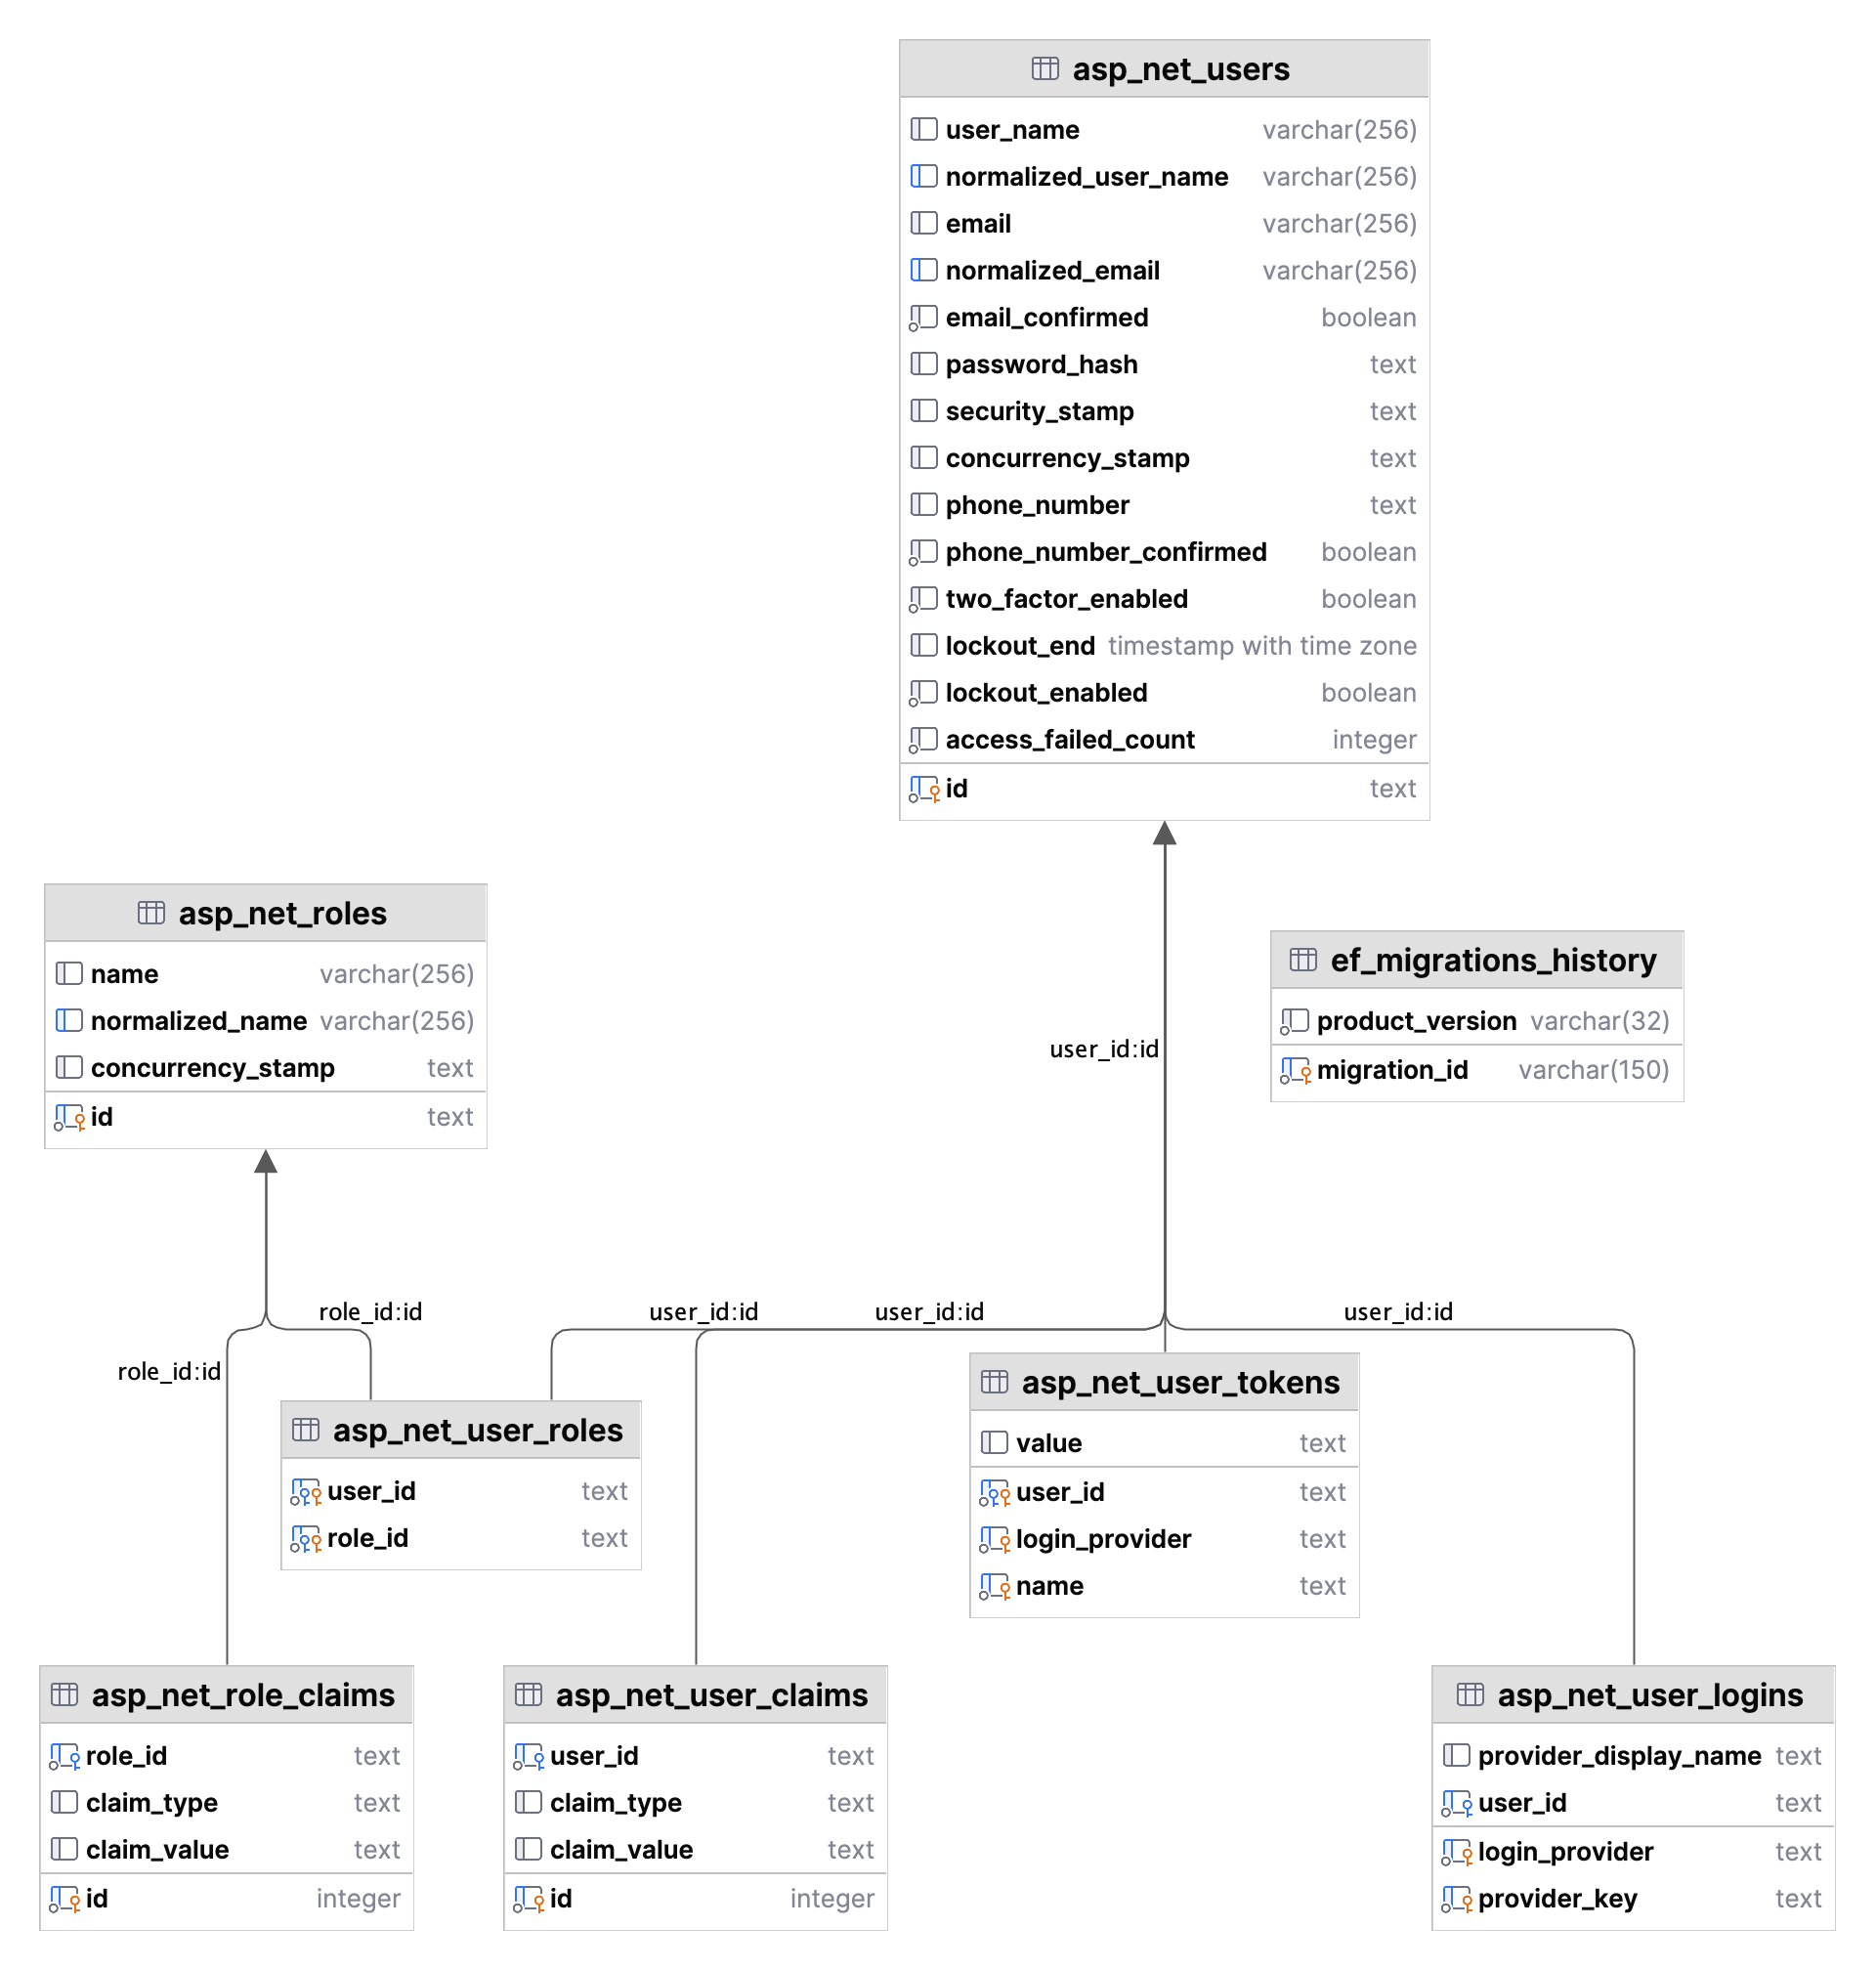
\includegraphics[width=1\textwidth]{attachments/user_data}
\caption{Diagram ERD schematu user\_data}
\label{fig:figure}
\end{figure}

\subsubsection{Tabela \keyword{ef\_migrations\_history}}
Tabela przechowuje historię migracji bazy danych.
\begin{itemize}
    \item \keyword{migration\_id}: \keyword{varchar(150)}, klucz główny, nie może być \keyword{NULL}
    \item \keyword{product\_version}: \keyword{varchar(32)}, nie może być \keyword{NULL}
\end{itemize}

\subsubsection{Tabela \keyword{asp\_net\_roles}}
Tabela przechowuje informacje o rolach użytkowników.
\begin{itemize}
    \item \keyword{id}: \keyword{text}, klucz główny, nie może być \keyword{NULL}
    \item \keyword{name}: \keyword{varchar(256)}
    \item \keyword{normalized\_name}: \keyword{varchar(256)}
    \item \keyword{concurrency\_stamp}: \keyword{text}
\end{itemize}
Indeksy:
\begin{itemize}
    \item \keyword{RoleNameIndex} na kolumnie \keyword{normalized\_name} (unikatowy)
\end{itemize}

\subsubsection{Tabela \keyword{asp\_net\_users}}
Tabela przechowuje informacje o użytkownikach.
\begin{itemize}
    \item \keyword{id}: \keyword{text}, klucz główny, nie może być \keyword{NULL}
    \item \keyword{user\_name}: \keyword{varchar(256)}
    \item \keyword{normalized\_user\_name}: \keyword{varchar(256)}
    \item \keyword{email}: \keyword{varchar(256)}
    \item \keyword{normalized\_email}: \keyword{varchar(256)}
    \item \keyword{email\_confirmed}: \keyword{boolean}, nie może być \keyword{NULL}
    \item \keyword{password\_hash}: \keyword{text}
    \item \keyword{security\_stamp}: \keyword{text}
    \item \keyword{concurrency\_stamp}: \keyword{text}
    \item \keyword{phone\_number}: \keyword{text}
    \item \keyword{phone\_number\_confirmed}: \keyword{boolean}, nie może być \keyword{NULL}
    \item \keyword{two\_factor\_enabled}: \keyword{boolean}, nie może być \keyword{NULL}
    \item \keyword{lockout\_end}: \keyword{timestamp with time zone}
    \item \keyword{lockout\_enabled}: \keyword{boolean}, nie może być \keyword{NULL}
    \item \keyword{access\_failed\_count}: \keyword{integer}, nie może być \keyword{NULL}
\end{itemize}
Indeksy:
\begin{itemize}
    \item \keyword{EmailIndex} na kolumnie \keyword{normalized\_email}
    \item \keyword{UserNameIndex} na kolumnie \keyword{normalized\_user\_name} (unikatowy)
\end{itemize}

\subsubsection{Tabela \keyword{asp\_net\_role\_claims}}
Tabela przechowuje informacje o roszczeniach przypisanych do ról.
\begin{itemize}
    \item \keyword{id}: \keyword{integer}, generowany automatycznie, klucz główny
    \item \keyword{role\_id}: \keyword{text}, nie może być \keyword{NULL}, klucz obcy od \keyword{asp\_net\_roles}, kaskadowe usuwanie
    \item \keyword{claim\_type}: \keyword{text}
    \item \keyword{claim\_value}: \keyword{text}
\end{itemize}
Indeksy:
\begin{itemize}
    \item \keyword{ix\_asp\_net\_role\_claims\_role\_id} na kolumnie \keyword{role\_id}
\end{itemize}

\subsubsection{Tabela \keyword{asp\_net\_user\_claims}}
Tabela przechowuje informacje o roszczeniach przypisanych do użytkowników.
\begin{itemize}
    \item \keyword{id}: \keyword{integer}, generowany automatycznie, klucz główny
    \item \keyword{user\_id}: \keyword{text}, nie może być \keyword{NULL}, klucz obcy od \keyword{asp\_net\_users}, kaskadowe usuwanie
    \item \keyword{claim\_type}: \keyword{text}
    \item \keyword{claim\_value}: \keyword{text}
\end{itemize}
Indeksy:
\begin{itemize}
    \item \keyword{ix\_asp\_net\_user\_claims\_user\_id} na kolumnie \keyword{user\_id}
\end{itemize}

\subsubsection{Tabela \keyword{asp\_net\_user\_logins}}
Tabela przechowuje informacje o logowaniach użytkowników.
\begin{itemize}
    \item \keyword{login\_provider}: \keyword{text}, nie może być \keyword{NULL}
    \item \keyword{provider\_key}: \keyword{text}, nie może być \keyword{NULL}
    \item \keyword{provider\_display\_name}: \keyword{text}
    \item \keyword{user\_id}: \keyword{text}, nie może być \keyword{NULL}, klucz obcy od \keyword{asp\_net\_users}, kaskadowe usuwanie
    \item Klucz główny: (\keyword{login\_provider}, \keyword{provider\_key})
\end{itemize}
Indeksy:
\begin{itemize}
    \item \keyword{ix\_asp\_net\_user\_logins\_user\_id} na kolumnie \keyword{user\_id}
\end{itemize}

\subsubsection{Tabela \keyword{asp\_net\_user\_roles}}
Tabela przechowuje informacje o przypisaniu ról do użytkowników.
\begin{itemize}
    \item \keyword{user\_id}: \keyword{text}, nie może być \keyword{NULL}, klucz obcy od \keyword{asp\_net\_users}, kaskadowe usuwanie
    \item \keyword{role\_id}: \keyword{text}, nie może być \keyword{NULL}, klucz obcy od \keyword{asp\_net\_roles}, kaskadowe usuwanie
    \item Klucz główny: (\keyword{user\_id}, \keyword{role\_id})
\end{itemize}
Indeksy:
\begin{itemize}
    \item \keyword{ix\_asp\_net\_user\_roles\_role\_id} na kolumnie \keyword{role\_id}
\end{itemize}

\subsubsection{Tabela \keyword{asp\_net\_user\_tokens}}
Tabela przechowuje informacje o tokenach użytkowników.
\begin{itemize}
    \item \keyword{user\_id}: \keyword{text}, nie może być \keyword{NULL}, klucz obcy od \keyword{asp\_net\_users}, kaskadowe usuwanie
    \item \keyword{login\_provider}: \keyword{text}, nie może być \keyword{NULL}
    \item \keyword{name}: \keyword{text}, nie może być \keyword{NULL}
    \item \keyword{value}: \keyword{text}
    \item Klucz główny: (\keyword{user\_id}, \keyword{login\_provider}, \keyword{name})
\end{itemize}

\subsection{Schemat \texttt{data}}

\begin{figure}[H]
\centering
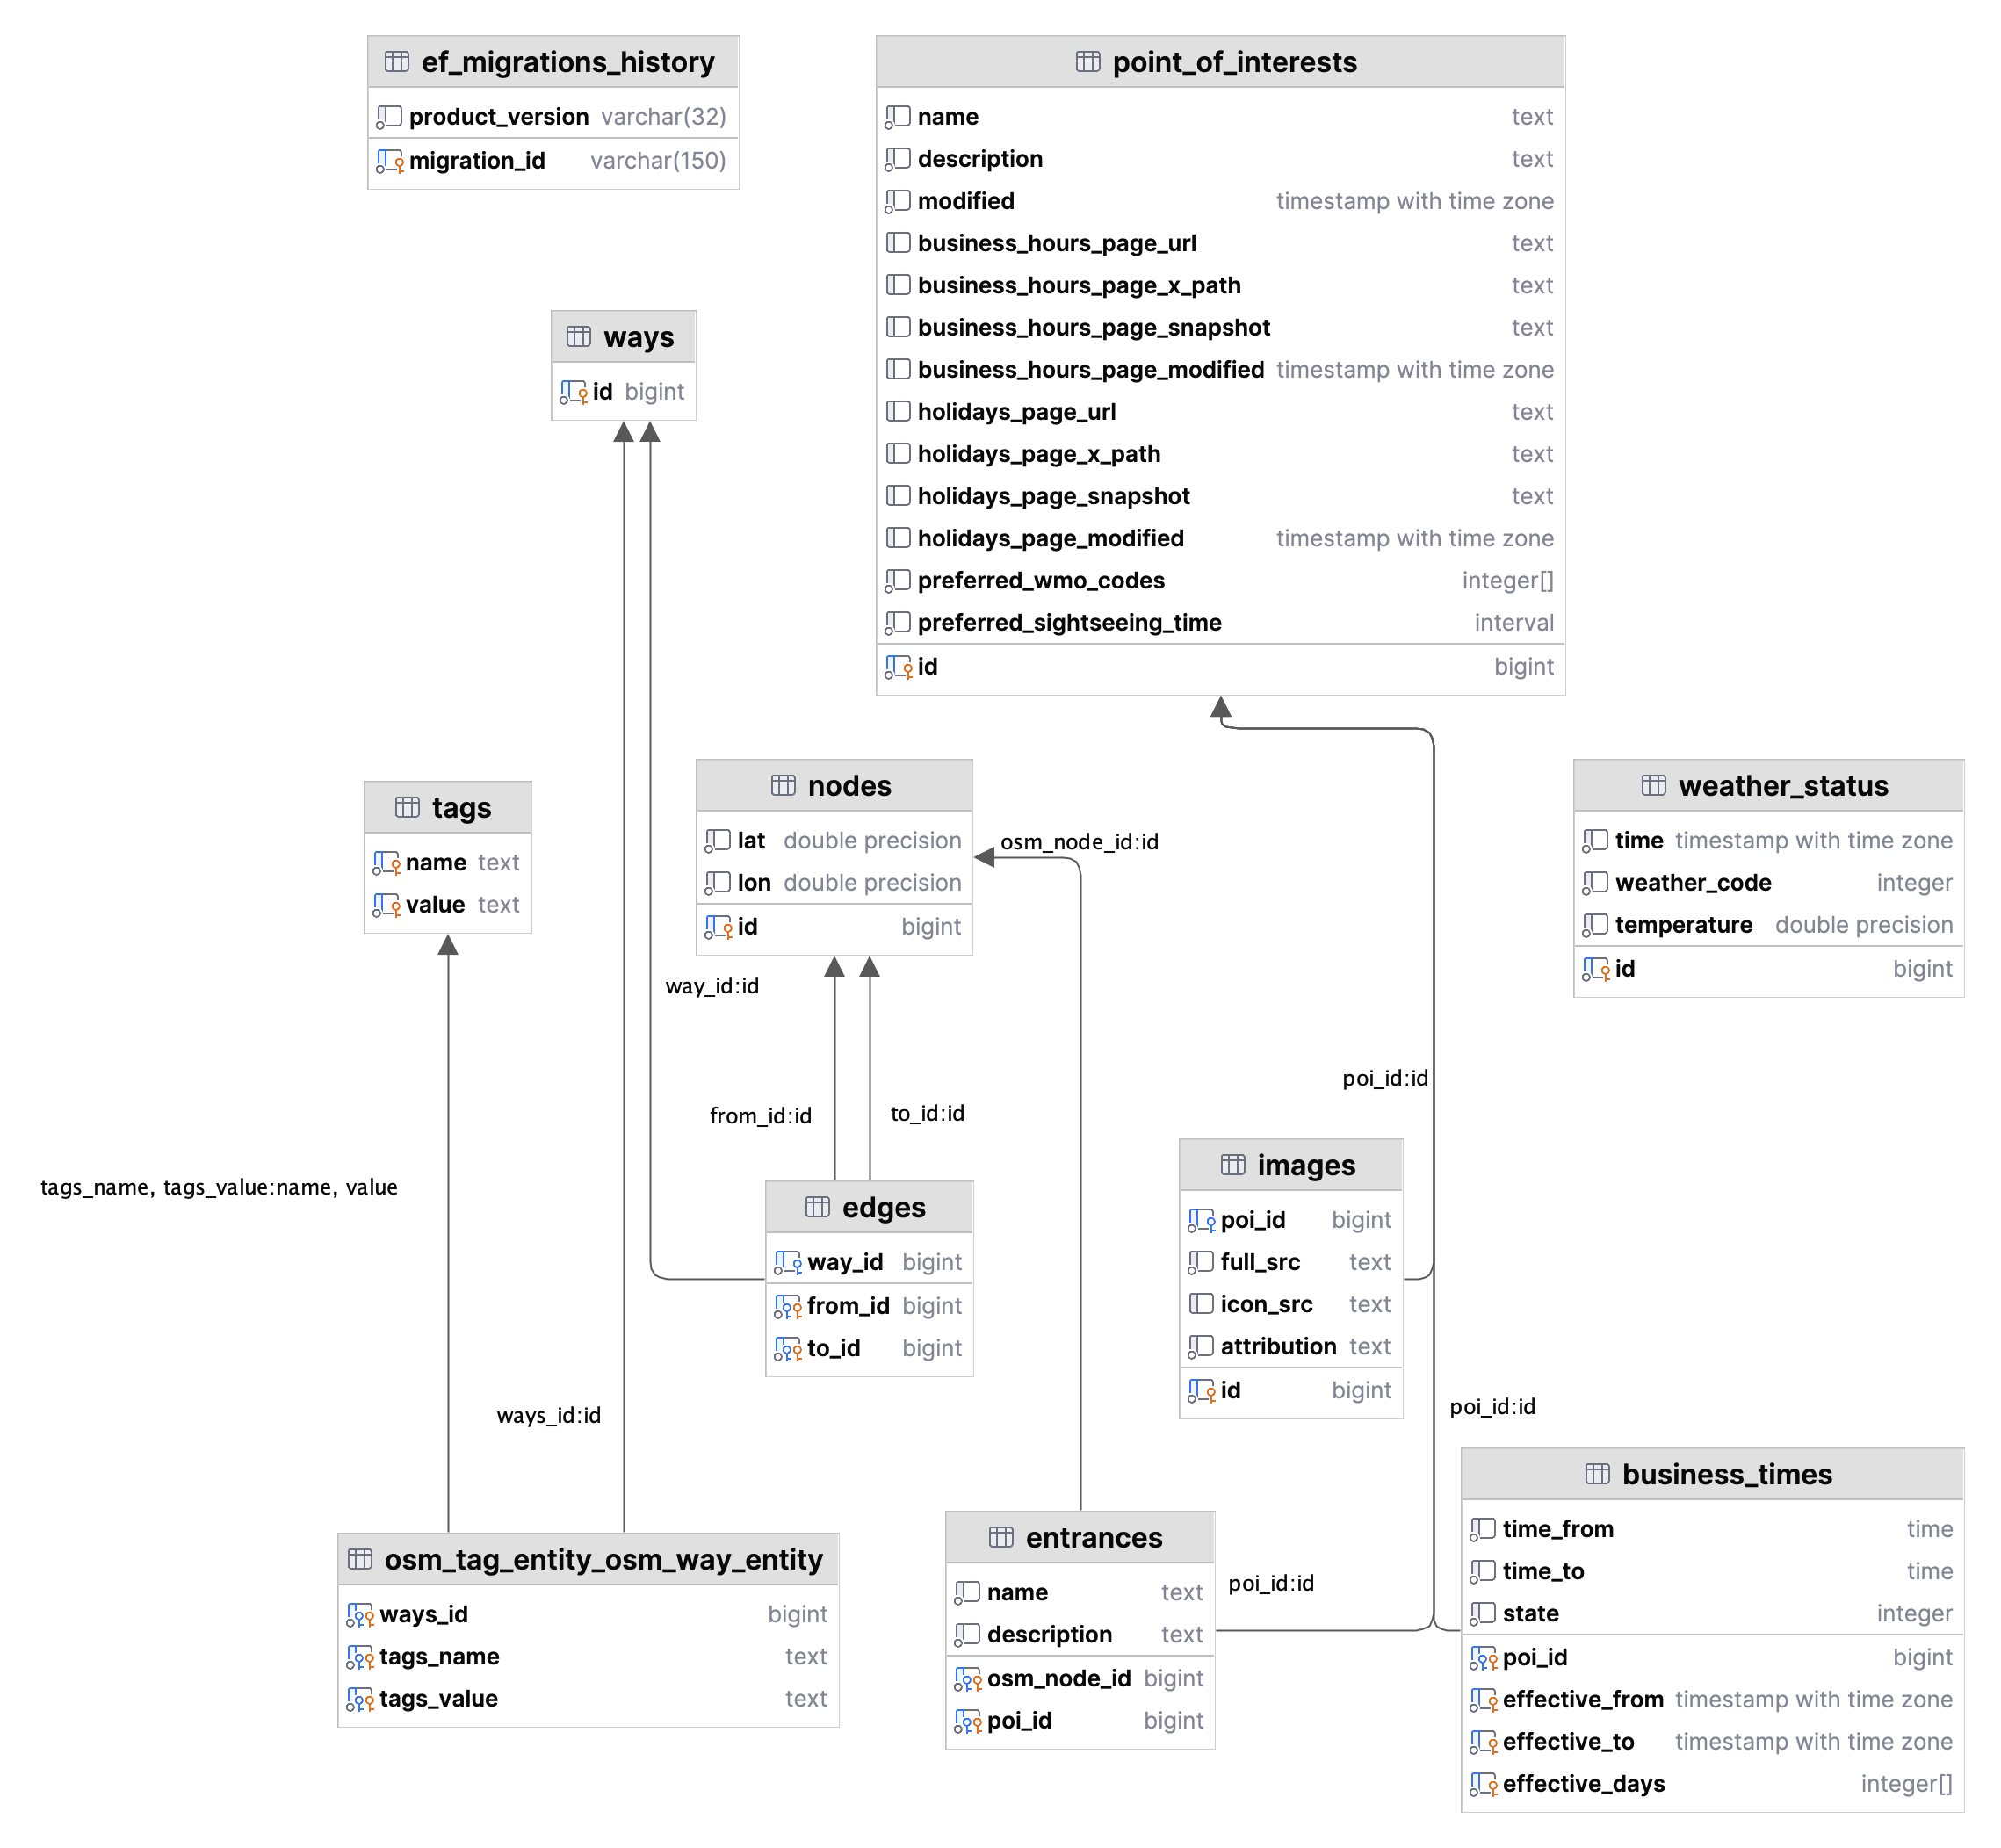
\includegraphics[width=1\textwidth]{attachments/data}
\caption{Diagram ERD schematu data}
\label{fig:figure}
\end{figure}

\subsubsection{Tabela \keyword{ef\_migrations\_history}}
Tabela przechowuje historię migracji bazy danych.
\begin{itemize}
    \item \keyword{migration\_id}: \keyword{varchar(150)}, klucz główny, nie może być \keyword{NULL}
    \item \keyword{product\_version}: \keyword{varchar(32)}, nie może być \keyword{NULL}
\end{itemize}

\subsubsection{Tabela \keyword{nodes}}
Tabela przechowuje informacje o węzłach, w tym ich identyfikator oraz współrzędne geograficzne.
\begin{itemize}
    \item \keyword{id}: \keyword{bigint}, klucz główny, nie może być \keyword{NULL}
    \item \keyword{lat}: \keyword{double precision}, nie może być \keyword{NULL}
    \item \keyword{lon}: \keyword{double precision}, nie może być \keyword{NULL}
\end{itemize}

\subsubsection{Tabela \keyword{point\_of\_interests}}
Tabela przechowuje informacje o punktach zainteresowania, takich jak nazwa, opis oraz godziny otwarcia.
\begin{itemize}
    \item \keyword{id}: \keyword{bigint}, generowany automatycznie, klucz główny
    \item \keyword{name}: \keyword{text}, nie może być \keyword{NULL}
    \item \keyword{description}: \keyword{text}, nie może być \keyword{NULL}
    \item \keyword{modified}: \keyword{timestamp with time zone}, nie może być \keyword{NULL}
    \item \keyword{business\_hours\_page\_url}: \keyword{text}, może być \keyword{NULL}
    \item \keyword{business\_hours\_page\_x\_path}: \keyword{text}, może być \keyword{NULL}
    \item \keyword{business\_hours\_page\_snapshot}: \keyword{text}, może być \keyword{NULL}
    \item \keyword{business\_hours\_page\_modified}: \keyword{timestamp with time zone}, może być \keyword{NULL}
    \item \keyword{holidays\_page\_url}: \keyword{text}, może być \keyword{NULL}
    \item \keyword{holidays\_page\_x\_path}: \keyword{text}, może być \keyword{NULL}
    \item \keyword{holidays\_page\_snapshot}: \keyword{text}, może być \keyword{NULL}
    \item \keyword{holidays\_page\_modified}: \keyword{timestamp with time zone}, może być \keyword{NULL}
    \item \keyword{preferred\_wmo\_codes}: \keyword{integer[]}, nie może być \keyword{NULL}
    \item \keyword{preferred\_sightseeing\_time}: \keyword{interval}, nie może być \keyword{NULL}
\end{itemize}

\subsubsection{Tabela \keyword{tags}}
Tabela przechowuje tagi używane do opisywania różnych encji.
\begin{itemize}
    \item \keyword{name}: \keyword{text}, nie może być \keyword{NULL}
    \item \keyword{value}: \keyword{text}, nie może być \keyword{NULL}
    \item Klucz główny: (\keyword{name}, \keyword{value})
\end{itemize}

\subsubsection{Tabela \keyword{ways}}
Tabela przechowuje informacje o drogach.
\begin{itemize}
    \item \keyword{id}: \keyword{bigint}, klucz główny, nie może być \keyword{NULL}
\end{itemize}

\subsubsection{Tabela \keyword{business\_times}}
Tabela przechowuje informacje o godzinach otwarcia dla punktów zainteresowania.
\begin{itemize}
    \item \keyword{poi\_id}: \keyword{bigint}, nie może być \keyword{NULL}, klucz obcy od \keyword{point\_of\_interests}, kaskadowe usuwanie
    \item \keyword{effective\_from}: \keyword{timestamp with time zone}, nie może być \keyword{NULL}
    \item \keyword{effective\_to}: \keyword{timestamp with time zone}, nie może być \keyword{NULL}
    \item \keyword{effective\_days}: \keyword{integer[]}, nie może być \keyword{NULL}
    \item \keyword{time\_from}: \keyword{time}, nie może być \keyword{NULL}
    \item \keyword{time\_to}: \keyword{time}, nie może być \keyword{NULL}
    \item \keyword{state}: \keyword{integer}, nie może być \keyword{NULL}
    \item Klucz główny: (\keyword{poi\_id}, \keyword{effective\_from}, \keyword{effective\_to}, \keyword{effective\_days})
\end{itemize}

\subsubsection{Tabela \keyword{entrances}}
Tabela przechowuje informacje o wejściach do punktów zainteresowania.
\begin{itemize}
    \item \keyword{osm\_node\_id}: \keyword{bigint}, nie może być \keyword{NULL}, klucz obcy od \keyword{nodes}, kaskadowe usuwanie
    \item \keyword{poi\_id}: \keyword{bigint}, nie może być \keyword{NULL}, klucz obcy od \keyword{point\_of\_interests}, kaskadowe usuwanie
    \item \keyword{name}: \keyword{text}, nie może być \keyword{NULL}
    \item \keyword{description}: \keyword{text}, nie może być \keyword{NULL}
    \item Klucz główny: (\keyword{osm\_node\_id}, \keyword{poi\_id})
\end{itemize}
Indeksy:
\begin{itemize}
    \item \keyword{ix\_entrances\_poi\_id} na kolumnie \keyword{poi\_id}
\end{itemize}

\subsubsection{Tabela \keyword{images}}
Tabela przechowuje informacje o obrazach związanych z punktami zainteresowania.
\begin{itemize}
    \item \keyword{id}: \keyword{bigint}, generowany automatycznie, klucz główny
    \item \keyword{poi\_id}: \keyword{bigint}, nie może być \keyword{NULL}, klucz obcy od \keyword{point\_of\_interests}, kaskadowe usuwanie
    \item \keyword{full\_src}: \keyword{text}, nie może być \keyword{NULL}
    \item \keyword{icon\_src}: \keyword{text}, może być \keyword{NULL}
    \item \keyword{attribution}: \keyword{text}, nie może być \keyword{NULL}
\end{itemize}
Indeksy:
\begin{itemize}
    \item \keyword{ix\_images\_poi\_id} na kolumnie \keyword{poi\_id}
\end{itemize}

\subsubsection{Tabela \keyword{edges}}
Tabela przechowuje informacje o połączeniach między węzłami.
\begin{itemize}
    \item \keyword{from\_id}: \keyword{bigint}, nie może być \keyword{NULL}, klucz obcy od \keyword{nodes}, kaskadowe usuwanie
    \item \keyword{to\_id}: \keyword{bigint}, nie może być \keyword{NULL}, klucz obcy od \keyword{nodes}, kaskadowe usuwanie
    \item \keyword{way\_id}: \keyword{bigint}, nie może być \keyword{NULL}, klucz obcy od \keyword{ways}, kaskadowe usuwanie
    \item Klucz główny: (\keyword{from\_id}, \keyword{to\_id})
\end{itemize}
Indeksy:
\begin{itemize}
    \item \keyword{ix\_edges\_to\_id} na kolumnie \keyword{to\_id}
    \item \keyword{ix\_edges\_way\_id} na kolumnie \keyword{way\_id}
\end{itemize}

\subsubsection{Tabela \keyword{osm\_tag\_entity\_osm\_way\_entity}}
Tabela przechowuje informacje o tagach przypisanych do dróg.
\begin{itemize}
    \item \keyword{ways\_id}: \keyword{bigint}, nie może być \keyword{NULL}, klucz obcy od \keyword{ways}, kaskadowe usuwanie
    \item \keyword{tags\_name}: \keyword{text}, nie może być \keyword{NULL}
    \item \keyword{tags\_value}: \keyword{text}, nie może być \keyword{NULL}
    \item Klucz główny: (\keyword{ways\_id}, \keyword{tags\_name}, \keyword{tags\_value})
    \item Klucz obcy: (\keyword{tags\_name}, \keyword{tags\_value}) odnosi się do \keyword{tags}, kaskadowe usuwanie
\end{itemize}
Indeksy:
\begin{itemize}
    \item \keyword{ix\_osm\_tag\_entity\_osm\_way\_entity\_tags\_name\_tags\_value} na kolumnach \keyword{tags\_name}, \keyword{tags\_value}
\end{itemize}

\subsection{Uprawnienia}
Wszystkie tabele i sekwencje są przypisane do właściciela \keyword{city\_planner\_user}.
Użytkownik \keyword{city\_planner\_user} ma szerokie uprawnienia (\keyword{delete}, \keyword{insert}, \keyword{references}, \keyword{select}, \keyword{trigger}, \keyword{truncate}, \keyword{update}) na wszystkich tabelach oraz wybrane uprawnienia na sekwencjach (\keyword{select}, \keyword{update}, \keyword{usage}).

\section{Frontend}
Frontend został wykonany w technologii Angular 17, korzystając z języka TypeScript w wersji 5.4 oraz biblioteki RxJs w wersji 7.
Aplikacja wykorzystuje różne wzorce projektowe, takie jak MVVM (Model-View-ViewModel), który oddziela logikę biznesową od interfejsu użytkownika, MVC (Model-View-Controller), który strukturalnie rozdziela dane aplikacji, logikę i interfejs użytkownika, oraz Dependency Injection, czyli wstrzykiwanie zależności, co pozwala na bardziej elastyczne zarządzanie zależnościami w aplikacji.
Dodatkowo, za implementację stanu aplikacji odpowiada wzorzec Redux, który zapewnia centralne zarządzanie stanem aplikacji i ułatwia debugowanie oraz testowanie kodu.
